\documentclass[conference,letterpaper,onecolumn]{IEEEtran}
%\usepackage[latin1]{inputenc}
%\usepackage[ansinew]{inputenc}
\usepackage[utf8]{inputenc}

\usepackage{graphicx}
\usepackage{psfrag}
\usepackage{stfloats}
%\usepackage[spanish]{babel}
\usepackage{epsfig}
\usepackage{pifont}
\usepackage{amssymb}
\usepackage{fixltx2e}
\usepackage{amsmath}
\usepackage{rotate}
\usepackage{anysize}
%\usepackage{rotating}
%\usepackage{fancybox}
\usepackage{float}
\usepackage{fancybox}
\usepackage{subfig}

\newcommand{\pig}[1]{\mbox{\boldmath ${#1}$}	}

\newtheorem{Theod}{{\bf Definici\'on}}

\setlength{\oddsidemargin}{5mm}
\setlength{\evensidemargin}{5mm}
\setlength{\topmargin}{4mm}
\setlength{\textwidth}{15cm}
\setlength{\columnsep}{5mm}
\setlength{\textheight}{24cm}

\begin{document}

\title{Powering multiparameter homotopy-based simulation with a fast path following technique}

\author{\authorblockN{H\'ector V\'azquez-Leal$^1$, Roberto Casta\~neda-Sheissa$^1$, Felipe Rabago-Bernal$^2$, Luis Hern\'andez-Mart\'inez$^3$,\\ Arturo Sarmiento-Reyes$^3$, Uriel Filobello-Ni\~no$^1$}
\authorblockA{$^1$University of Veracruz\\
Electronic Instrumentation and Atmospheric Sciences School\\
Xalapa, Veracruz, M\'exico\\
E-mail: hvazquez@uv.mx, rocastaneda@uv.mx, ufilobello@uv.mx\\
$^2$ Autonomous University of San Luis Potosi\\
Physics Institute\\
San Luis Potosi, San Luis Potosi, M\'exico\\
E-mail: rabago@dec1.ifisica.uaslp.mx\\
$^3$ National Institute for Astrophisics, Optics and Electronics\\
Electronics Department\\
Tonantzintla, Puebla, M\'exico\\
E-mail: luish@inaoep.mx, jarocho@inaoep.mx}
}

\maketitle

\begin{abstract}
The continuous scaling for fabrication technologies of electronic circuits demands the design of new and improved simulation techniques for integrated circuits. Therefore,
this work shows how the hypersphere technique can be adapted and applied to trace a multiparameter homotopy. Besides, we present a path following technique based in circles (evolved from hypersphere), which is faster, and simpler to be implemented than hypersphere technique. Last, a comparative analysis between both techniques applied to simulation of circuits with bipolar transistors will be shown.
\end{abstract}
 
\section{Introduction} 
The increment of the complexity of circuits impulse the scientific progress in the simulation techniques area for integrated circuits. Also, homotopy techniques have been introduced as a useful tool in the area of operating point solution for circuits \cite{homo_green05,homo_ArtificialP,homo_coercitivo,homo_iscas05,homo_MOS}, due to the Newton-Raphson (NR) method (widely used) shows convergence problems \cite{NEWTONR} like oscillation and divergence.

\section{Multiparameter homotopy}
The first step to formulate a homotopy is to establish the equilibrium equation to be solved; it is formulated from kirchhoff laws, being defined as:

\begin{equation}
{f}({x})={0} \qquad \text{where} \qquad f:\in \mathfrak{R}^n \to  \mathfrak{R}^n, 
\label{fx}
\end{equation}
where $x$ represents the electrical variables of the circuit and $n$ is the number of electrical variables.

Multiparameter Homotopies \cite{homo_DWolfMulti,BLHOM2,homo_dobletrazado} are characterized for adding more than one extra homotopy parameter to the equilibrium equation. When homotopy parameters are adjusted to zero, the solution for $H(\cdot)$ becomes trivial and when parameters reach value of one, then the operating point is located. The multiparameter homotopy function can be represented as:

\begin{equation}
{H}({f}({x}),\lambda_1,\lambda_2,...,\lambda_k)=0, 
\end{equation}
where homotopy parameters are $\lambda_1,\lambda_2,...\lambda_k\in[0,1]$ and $k$ is the number of homotopy parameters.

Multiparameter homotopy \cite{homo_DWolfMulti} has been proposed in order to avoid fork bifurcations, singularities, among other problems that can be encountered with homotopy paths. Besides, as for the uniparametric \cite{homo_ArtificialP} and multiparameter homotopies, the tracing technique \cite{homo_hk,homo_allgower} is a fundamental tool capable to affect the convergence, speed and number of solutions located. Therefore, it is proposed to apply two tracing techniques for multiparameter homotopy, both will be described in the following sections.

\section{Tracing techniques}
In order to apply tracing techniques described in this article, will be used as an example, a biparametric homotopy based in Newton's homotopy method:


\begin{equation}
{H}({f}({x}),\lambda_1,\lambda_2 ) =f(x,\lambda_2)-(1-\lambda_1 )f(x_i,0) \qquad \text{where} \qquad H:\in \mathfrak{R}^{n+1} \times \mathfrak{R} \to  \mathfrak{R}^n. 
\label{hexamp1l}
\end{equation}

With the existence of two parameters ($\lambda_1$ and $\lambda_2$), two simultaneous deformations or transformations are produced; one in function $f$ and another in function $H$. When $[x,\lambda_1,\lambda_2]=[x_i,0,0]$ then:
\begin{equation}
{H}({f}({x}),\lambda_1,\lambda_2 ) = f(x_i,0)-f(x_i,0)=0, 
\label{hexamp1l1}
\end{equation}
hence, homotopy function is satisfied. Besides, when $[\lambda_1,\lambda_2]=[1,1]$ becomes:
\begin{equation}
{H}({f}({x}),\lambda_1,\lambda_2 ) = f(x),
\label{hexamp1l2}
\end{equation}
so the found solution of $H$ is the solution of the equilibrium equation. Nonetheless, as function $H$ has two extra variables, it is necessary to add two equations to the system $H$ in order to be solved using more conventional techniques like NR.

\begin{enumerate}
\item {\bf Equation $n+1$}. One equation is added to define path $\lambda_1-\lambda_2$, which will be named parametric function $M(\lambda_1,\lambda_2)$. This equation traverses three points $[\lambda_1,\lambda_2]$: $p_1=[0,0]$, $p_2=[A,B]$, and $p_3=[1,1]$. The proposed equation is:

{\large
\begin{equation}
\begin{array}{c}
M(\lambda_1,\lambda_2)= {\LARGE-\lambda_{{1}}+{ \left( \lambda_{{2}}+{\frac {B \left( - 1+A \right) }
{AB+ 1- 2A}} \right) \over  \left( -{\frac { \left( - 1+ 2\,
A- B \right) \lambda_{{2}}}{AB+ 1- 2A}}+ 2\,{\frac {B
 \left( - 1+A \right) }{AB+ 1- 2A}} \right) }},
\end{array}
\label{homotopiaPx4}
\end{equation}
}
where $p_2$ is defined by user, as shown in Fig. \ref{curvasl}(a). The range of values for $A$ and $B$ is $[0,1]$.

\item {\bf Equation $n+2$}. Hypersphere equation is added \cite{hiper}:

{
\begin{equation}
\begin{array}{c}
S(\cdot)=(x_1-c_1)^2+ (x_2-c_2)^2+ \cdots+ (\lambda_1-c_{n+1})^2+(\lambda_2-c_{n+2})^2-r^2,
\end{array}
\label{hiperesfera}
\end{equation}
}
where $\pig{c}$ is the center of the hypersphere (which adjusts its value each iteration) and $r\ll 1$ is the hypersphere radius (step size).
\end{enumerate}

\begin{figure}[hbtp]
\centering
\begin{minipage}{\linewidth}
\psfrag{l1}{$\lambda_2$}
\psfrag{l2}{$\lambda_1$}
\psfrag{p1}{$p_1=[0,0]$}
\psfrag{p2}{$p_2=[A,B]$}
\psfrag{p3}{$p_3=[1,1]$}
\centering
	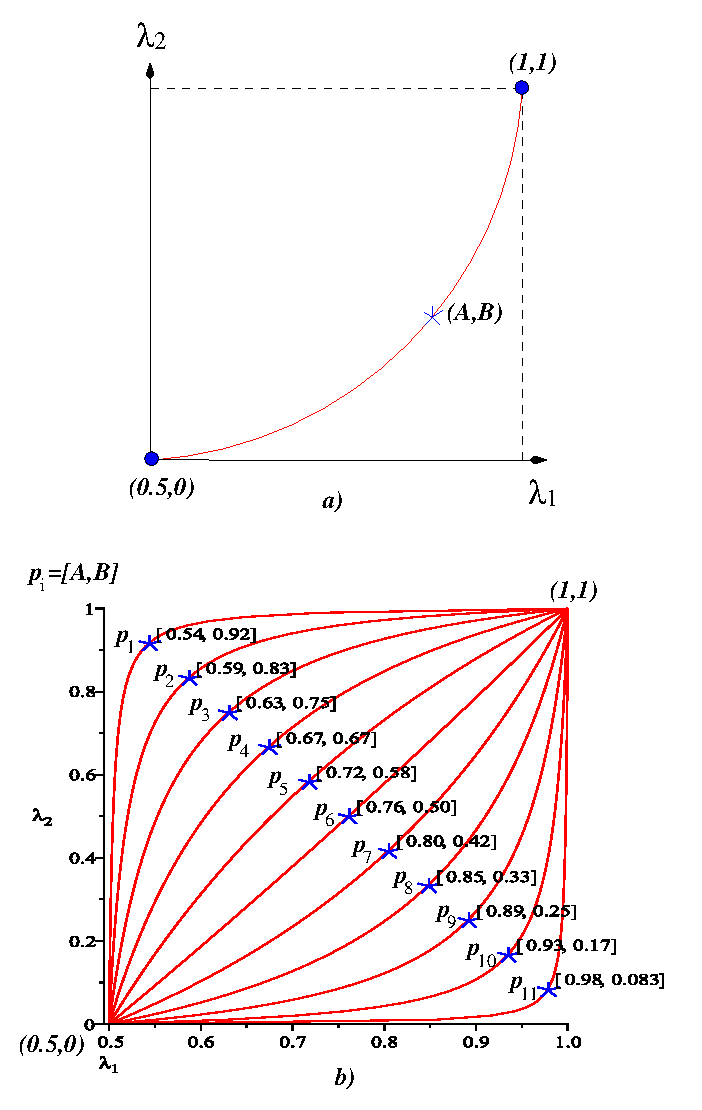
\includegraphics[scale=0.7]{fig/curvasl.eps}
\end{minipage}
\newline
\begin{minipage}{\linewidth}
\centering
(a) 
\end{minipage}
\newline
\newline
\begin{minipage}{\linewidth}
\centering
	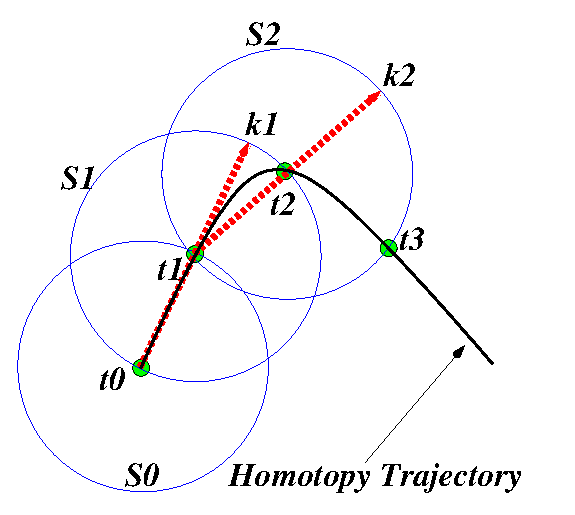
\includegraphics[scale=0.7]{fig/hiper.eps}
\end{minipage}
\newline
\begin{minipage}{\linewidth}
\centering
(b) 
\end{minipage}
\newline
\caption{a) Parametric function. b) Hypersphere technique.}
\label{curvasl}
\end{figure}

The summary of the procedures consists in the following steps \cite{hiper} (see Fig. \ref{curvasl}(b)):

\begin{enumerate}
\item The first sphere is established $S0$ with center located at $t0=[x_i,p_1]$ and the equation system is solved (equations (\ref{hexamp1l}), (\ref{homotopiaPx4}) and (\ref{hiperesfera})) using the NR method (setting $t0$ as initial point), locating point $t1$.
\item A new hypersphere $S1$ is created with center at $t1$.
\item Using points $t0$ and $t1$ it is possible to create a prediction, which touches hypersphere $S1$ at point $k_1$, it is used as initial point for the NR method, until locate point $t_2$ on the homotopy path.
\item Steps 2 and 3 are successively repeated (updating hypersphere's center after  each iteration) until crossing point $p_3$.
\item Points before and after $p_3$ are used to perform an interpolation \cite{homo_sosonkina}. The type of interpolation employed in this article is linear multidimensional interpolation, which produce an approximation $x_{a}$ of solution $x_s$ for the equilibrium equation.
\item Finally, using as initial point $x_a$ in the NR method, the precision for the operating point $x_s$ is improved.
\end{enumerate}

It is possible to replace equation \ref{hiperesfera} for the circle equation, in function of the homotopy parameters:

{
\begin{equation}
\begin{array}{c}
C(\cdot)=(\lambda_1-c_{n+1})^2+(\lambda_2-c_{n+2})^2-r^2,
\end{array}
\label{hiperesfera1}
\end{equation}}
where $r\ll 1$. The rest of the steps to implement the numerical continuation are the same as the hypersphere technique already described.

\section{Study case: Circuit with bipolar transistors and a diode}

The following circuit \cite{homo_chua} (see Fig. \ref{newchua}), contains nine solutions, has become the reference circuit for the homotopy applied to circuit analysis. Using the system reported by \cite{homo_chua}, equilibrium equation is augmented:

{ 
\begin{equation}
\pig{f}(v_1,v_2,v_3,v_4,\lambda_2)= \left\{
\begin{array}{ll}
f_1= 6.103168I_s(e^{40v_1}-1)\lambda_2+4.36634v_2\\ \,\qquad+2.863168I_s(e^{40v_2}-1)-12\\\\
f_2=5.4v_1+3.58I_s(e^{40v_1}-1)\lambda_2+6.62I_s(e^{40v_2}-1)\\ \,\qquad+v_3+0.7I_s(e^{40v_3}-1)+0.5I_s(e^{40v_4}-1)-22\\\\
f_3=6.103168I_s(e^{40v_3}-1)+2.863168I_s(e^{40v_4}-1)\lambda_2\\ \,\qquad+4.36634v_4-12\\\\
f_4=v_1+0.7I_s(e^{40v_1}-1)\lambda_2+0.5I_s(e^{40v_2}-1)+5.4v_3\\ \,\qquad+3.58I_s(e^{40v_3}-1)+6.62I_s(e^{40v_4}-1)\lambda_2-20 \\\\
\end{array}\right.
\label{fxl}
\end{equation}
}
 
\begin{figure}[hbtp]
\centering
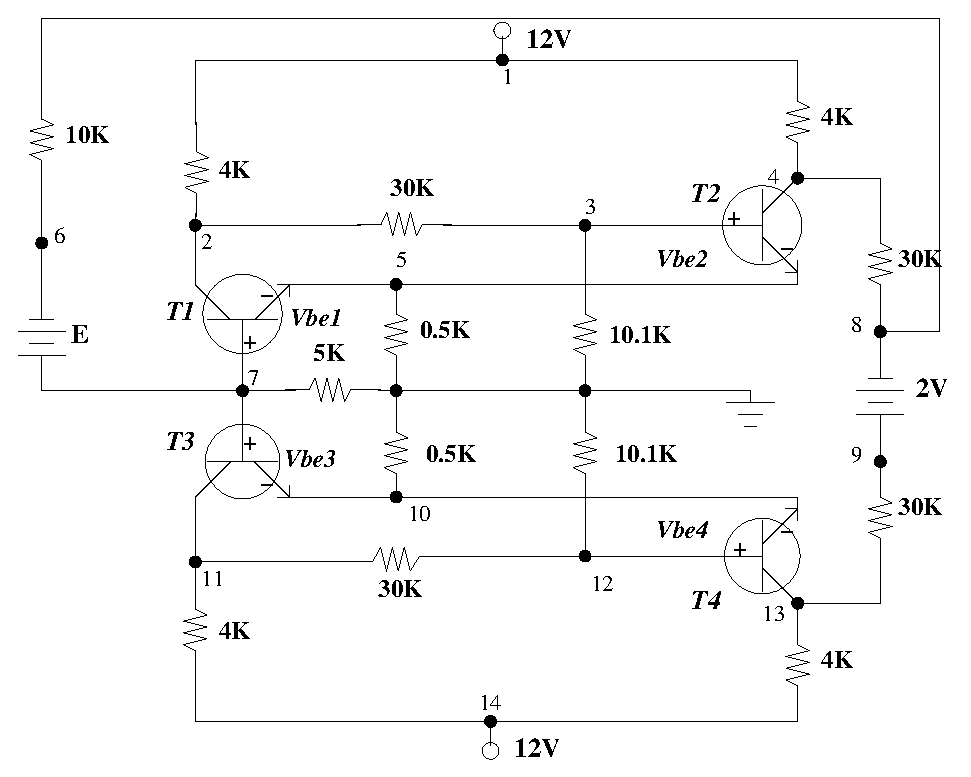
\includegraphics[scale=0.7]{fig/newchua.eps}
\caption{Chua's circuit.}
\label{newchua}
\end{figure}


where $I_s=10^{-6}$,  $[v_1,v_2,v_3, v_4]$ are the voltage drop between base-emitter terminals for each transistor in the circuit (see Fig. \ref{newchua}) and $\lambda_2$ is the second homotopy parameter. The complete homotopy formulation can be established by using equations:

\begin{itemize}
\item The augmented equilibrium equation (\ref{fxl}).
\item The homotopy function equation (\ref{hexamp1l}).
\item The parametric function (\ref{homotopiaPx4}).
\item The hypersphere function (\ref{hiperesfera}) or circle function (\ref{hiperesfera1}), it depends on the selected technique.
\end{itemize}

Table \ref{hs1} presents in summary the results of performing the tracing of four paths with different initial points ($x_{i1}$, $x_{i2}$, $x_{i3}$, and $x_{i4}$), each one. This process was repeated for both tracing techniques, showing the results in Fig. \ref{ht1} (a) and Fig. \ref{ht1}(b). Comparing both techniques, there are two interesting conclusions to be highlighted: first, homotopy paths traced from the same initial point leads to the same solution, in fact, comparing paths point by point it can be observed that it is the same path; second, despite that paths are identical, the circle technique required a fixed number of iterations (48), those are much less required than using the hypersphere method. In fact, from Table \ref{hs1} can be concluded that, at best (choosing initial point at $x_{i1}$), the tracing technique for circles required 8.95 times less CPU time (by using MAPLE 15 software in an Intel Quad Core i7 processor at 2.6 GHz) than the hypersphere technique. Both tracing techniques employed radius of $r=0.03$ and a parametric function $M$ with $p_2=[0.2,0.3]$.

\begin{table}[tbp]
\center{
\begin{large}
{\bf
\begin{tabular}{||c|c|c|c||}
\hline\hline
Hypersphere - Init. Point & \#  & Time & Operating Point $[v_1,v_2,v_3,v_4]$  \\ 
where $[\lambda_1,\lambda_2]=[0,0]$ & Iter & (Sec) &  where $[\lambda_1,\lambda_2]=[1,1]$\\ \hline \hline
$x_{i1}$=[-5, -5, -5, -5]  & 519 & 7.70 &$x_{s1}=$[0.3830, -3.5446, 0.3851, -4.0990] \\  \hline
$x_{i2}$=[-1, -2, -1, 0] & 202  & 3.59&$x_{s2}=$[0.3869, -4.6321, -0.8002, 0.3775] \\  \hline
$x_{i3}$=[-5, -0.5, -5, 0] & 216 &4.06& $x_{s3}=$[-0.5136, 0.3775, -0.9682, 0.3775] \\  \hline
$x_{i4}$=[-1, 0, 0, 0] & 168 & 3.13 &$x_{s4}=$[-1.0510, 0.3775, 0.3845, -3.9542]\\  \hline  \hline
Circle - Init. Point & \# & Time & Operating Point  $[v_1,v_2,v_3,v_4]$  \\ 
where $[\lambda_1,\lambda_2]=[0,0]$ & Iter & (Sec) & where $[\lambda_1,\lambda_2]=[1,1]$\\ \hline \hline
$x_{i1}$=[-5, -5, -5, -5]  & 48 & 0.86 & $x_{s1}=$[0.3830, -3.5446, 0.3851, -4.0990] \\  \hline
$x_{i2}$=[-1, -2, -1, 0] & 48  & 0.89 &$x_{s2}=$[0.3869, -4.6321, -0.8002, 0.3775] \\  \hline
$x_{i3}$=[-5, -0.5, -5, 0] & 48 & 0.74 & $x_{s4}=$[-0.5136, 0.3775, -0.9682, 0.3775] \\  \hline
$x_{i4}$=[-1, 0, 0, 0] & 48 & 0.82 &$x_{s4}=$[-1.0510, 0.3775, 0.3845, -3.9542]\\  \hline  \hline
\end{tabular}
}
\end{large}
}
\caption{Relevant points for homotopy simulations.}
\label{hs1}
\end{table}

\begin{figure}[!hbtp]
\centering
\begin{minipage}{\linewidth}
\centering
	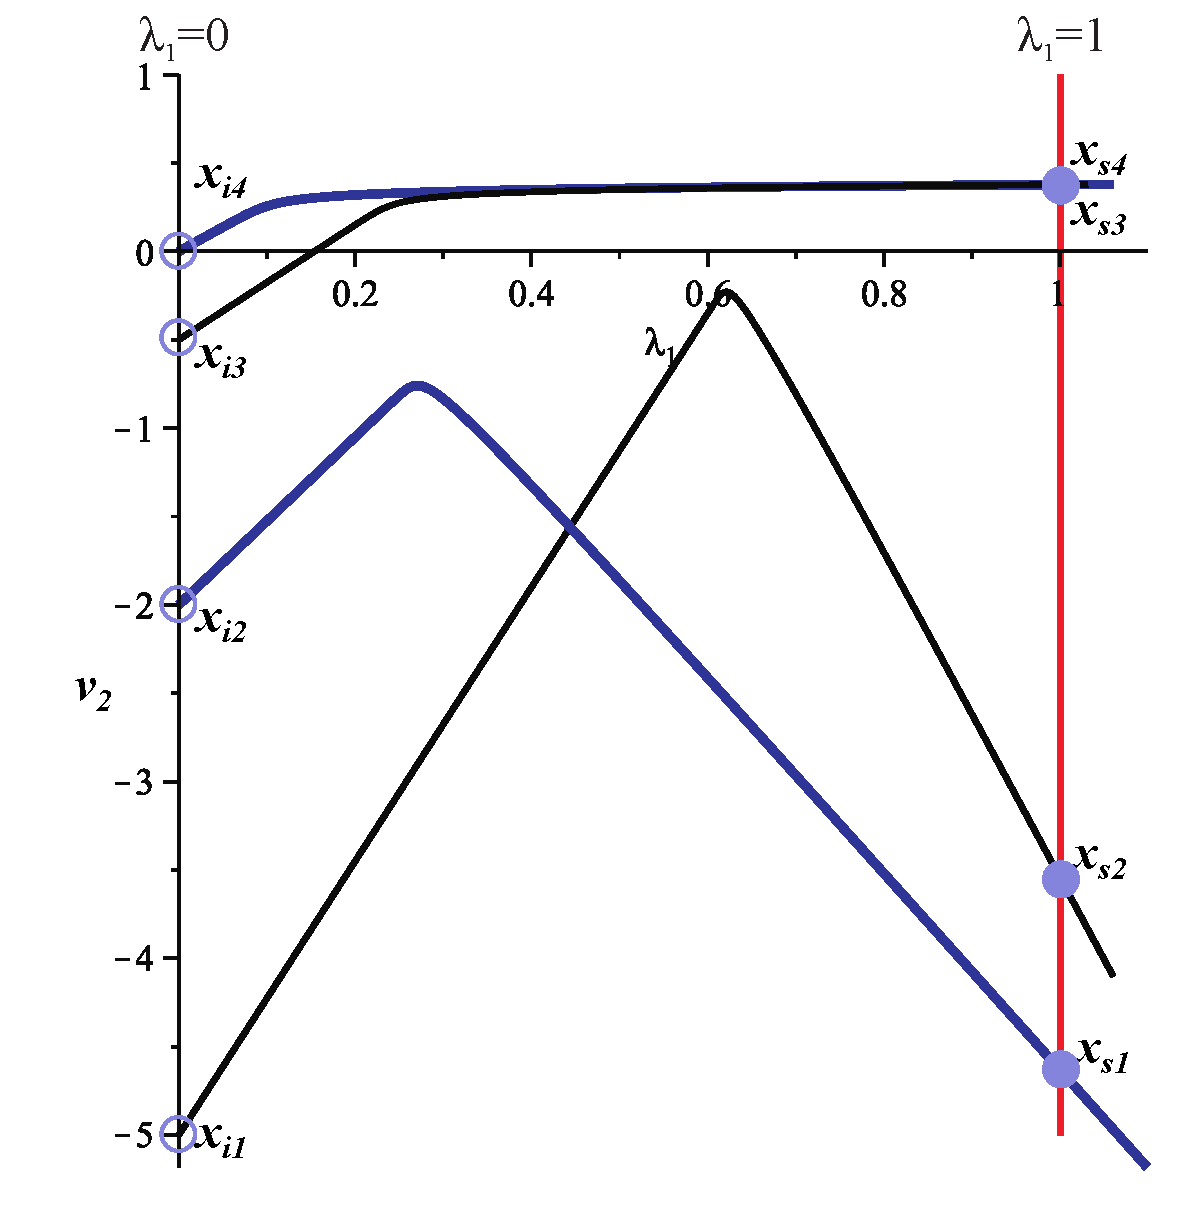
\includegraphics[scale=0.42]{fig/curvasesfera.eps}
\end{minipage}
\newline
\begin{minipage}{\linewidth}
\centering
(a) Hypersphere technique.
\end{minipage}
\newline
\newline
\begin{minipage}{\linewidth}
\centering
	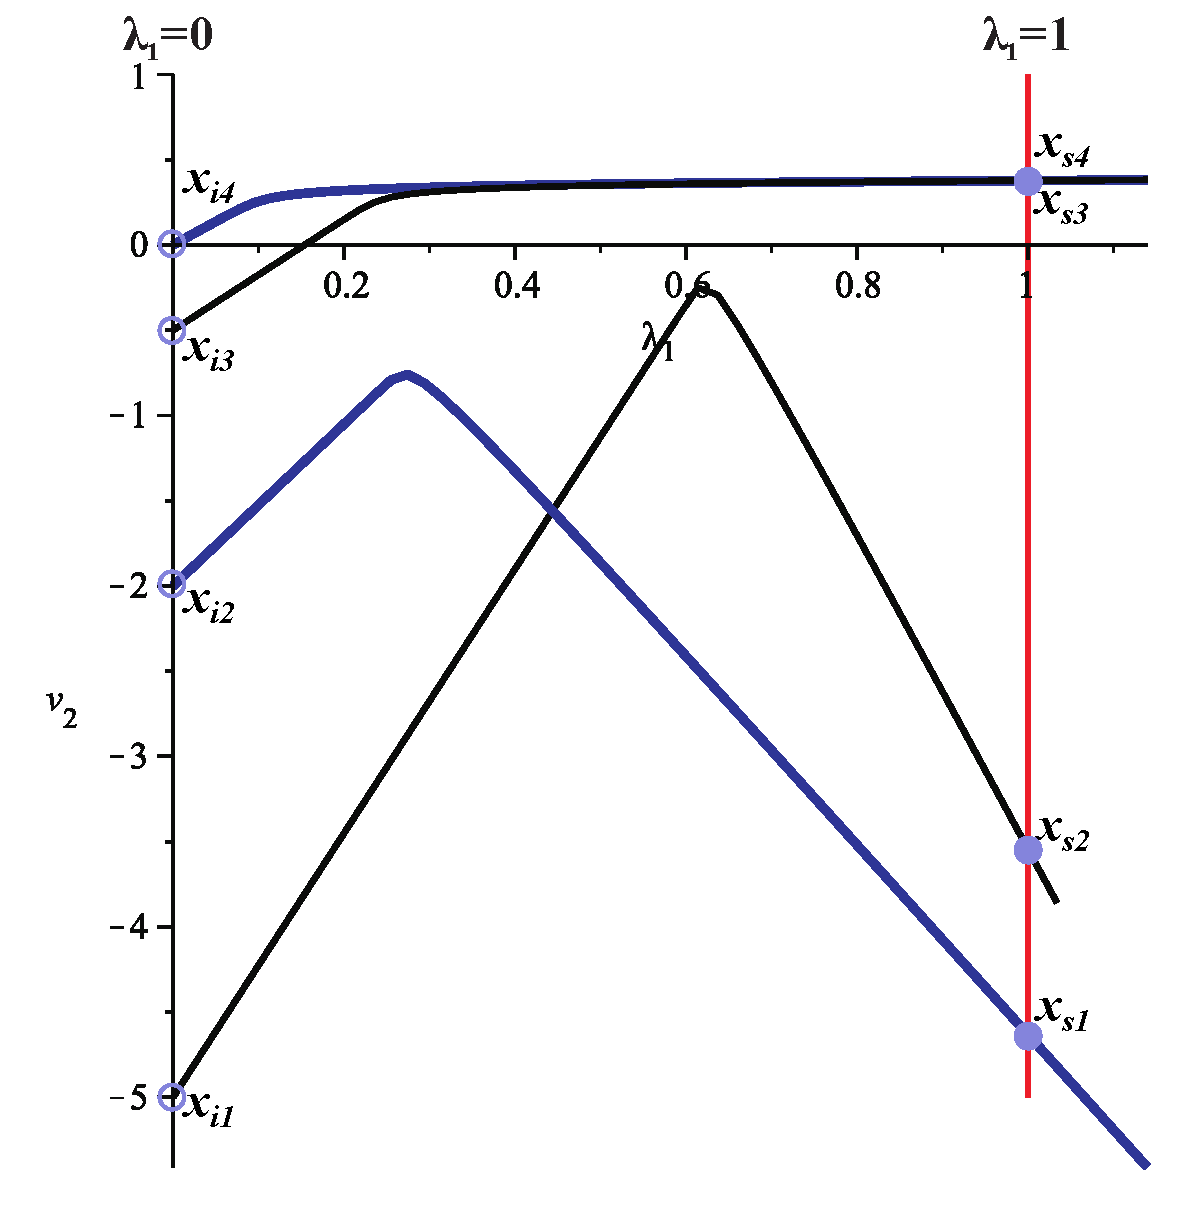
\includegraphics[scale=0.42]{fig/curvascirculo.eps}
\end{minipage}
\newline
\begin{minipage}{\linewidth}
\centering
(b) Circle technique.
\end{minipage}
\caption{Homotopy Trajectories $v_2-\lambda_1$.}
\label{ht1}
\end{figure}

Circles technique can be modified changing one of the homotopy parameters by an electrical variable of interest. For instance, the simulation was repeated from initial point $x_{i1}$, only changing the circle from equation (\ref{hiperesfera1}) by:

\begin{equation}
C(v_1,\lambda_1)=v_1^2+\lambda_1^2-r^2,
\end{equation}


where $v_1, r \in \Re$. The result was that the homotopy path already known was traced (see Fig. \ref{ht1}(b)) with a total of 191 iterations (locating the same solution at $x_{s1}$). Also, it is possible to use one of the two homotopy parameters with more than one electrical variable, to implement a reduced hypersphere. Therefore, in a forthcoming work the study  of circles technique will be expanded and a possible application to simulate VLSI circuits will also be discussed.

\section{Conclusion}
This work showed that it is possible to use the hypersphere technique to trace multiparameter Homotopies. Besides, a tracing technique derived from hypersphere (circles) was introduced; which is simpler to program and faster than the hypersphere technique. These results make the circles technique an attractive tool to trace multiparameter homotopies.

\bibliographystyle{unsrt}
\bibliography{nh5_eng}

\end{document}
